\documentclass[10pt]{article}
\usepackage[utf8]{inputenc}
\usepackage[T1]{fontenc}
\usepackage[english]{babel}
\usepackage{amsfonts}
\usepackage{amsmath}
\usepackage[pdftex]{color,graphicx}
\usepackage{pdfpages}
\usepackage{fancyhdr}
\usepackage{textcomp}
\usepackage{lmodern}
\usepackage{xcolor}
\usepackage{multicol}
\usepackage{soul}
\usepackage{url}
\usepackage{algorithmic}
\usepackage{wrapfig}
\usepackage{caption}
\usepackage{clrscode3e}
\usepackage{subcaption}
\usepackage{float}
\usepackage{mdwlist}
\usepackage{pgfgantt}
\usepackage[showframe=false]{geometry}
\usepackage{changepage}
\usepackage[bookmarks]{hyperref}
\usepackage{listings}
\usepackage{dirtree}
\usepackage{todonotes}
\pagestyle{fancy}
\usepackage[font=small,labelfont=bf]{caption}
\usepackage[dot, autosize, outputdir="dotgraphs/"]{dot2texi}
\usepackage{tikz}
\usetikzlibrary{shapes}
\usetikzlibrary{arrows,automata}


\newcommand{\HRule}{\rule{\linewidth}{0.5mm}}


\def\nosplit{\hfil\penalty 100 \hfilneg \hbox}

\newcommand{\myurl}[1]{\nosplit{\url{#1}}}
\newcommand{\graphicc}[4]{\begin{figure}[H] \centering
            \includegraphics[width={#1\textwidth}, keepaspectratio=true]{{#2}}
            \caption{{#3}} \label{#4} \end{figure}}
\newcommand{\norm}[1]{\left\lVert#1\right\rVert}

% Setup for lstlisting
\lstset{language=C++,
                basicstyle=\ttfamily,
                keywordstyle=\color{blue}\ttfamily,
                stringstyle=\color{red}\ttfamily,
                commentstyle=\color{green}\ttfamily,
                morecomment=[l][\color{magenta}]{\#}
}


\usepackage{tikz, xcolor}
\usetikzlibrary{shapes,arrows}


\tikzstyle{decision} = [diamond, draw, text width=4.5em, 
                        text badly centered, node distance=2cm, 
                        inner sep=0pt]
\tikzstyle{block} = [rectangle, draw, text width=5em, 
                     text centered, rounded corners, 
                     minimum height=4em, node distance=3cm]
\tikzstyle{line} = [draw, -latex']
\tikzstyle{cloud} = [draw, ellipse, node distance=2.5cm, minimum height=2em]
\tikzstyle{blank} = [node distance=1cm]
\tikzstyle{v1} = [node distance=1cm]


%If in need of a header for the document, uncomment this and add desired text!
\fancyhead[LO,LE]{Jenny V, Martin G \& Martin J}
\fancyhead[RO,RE]{Assignment 1, Advanced Algorithms and Datastructures}
%%%%%%%%%%%% END OF PREAMBLE %%%%%%%%%%%%%%%%%%%%%%%%%%%%%%%%%%%%
\begin{document}
\begin{titlepage}

\begin{center}

\textsc{\LARGE Assignment 1}\\%[1.5cm]

%\textsc{\Large Advanced Algorithms and Datastructures}\\[0.5cm]
%\textsc{\Large Jenny Vej, Martin Grunbaum \& Martin Jørgensen}\\[0.5cm]

\HRule \\[0.4cm]

%{ \bfseries\large Jenny Vej, Martin Grunbaum \& Martin Jørgensen}\\[1cm]
{ \bfseries\large Advanced Algorithms and Datastructures}\\[1cm]

\HRule \\ [7.5cm]

% Author and supervisor
\begin{minipage}{0.5\textwidth}
\begin{flushleft} \large
Authors:\\
Jenny-Margrethe Vej (rwj935)\\
Martin Gielsgaard Grünbaum (wrk272)\\
Martin Nicklas Jørgensen (tzk173)\\
\vspace{0.5cm}
\end{flushleft}
\end{minipage}
\begin{minipage}{0.4\textwidth}
\begin{flushright} {\large
\textbf{\today} }\\
\end{flushright}
\end{minipage}

\vfill

% Bottom of the page front page


\end{center}

\end{titlepage}
\clearpage

%\newpage
%\tableofcontents
%\newpage

\section{Hash functions for sampling}
\subsection{Exercise 1(a')}
We must show that $p \leq Pr[h_m(x)/m < p] \leq 1.01p$. To do so, we first
look at finding a different way to express the probability of sampling (i.e.\ probability
of $h_m(x)/m < p$). We then make use of various re-writes and the fact that $h_m$ is
strongly universal, to re-express the equality and find a tight bound.

We are given some $p \geq 100/m$, a suitably large $m$ and a strongly universal hashing
function $h_m : U \rightarrow [m]$. Note that $p \geq 100/m$ implies that $p/100 \geq 1/m$ 
and that for some generic $a$ (such as $pm$ in the following), $a \leq \lceil a \rceil < a+1$.

We observe that
\begin{align*}
	& Pr[h_m(x)/m < p] \\
	&= \sum_{0 \leq k < pm} Pr[h_m(x) = k] \\
	&= \sum_{0 \leq k < pm} \frac{1}{m} \\
	&= \frac{1}{m} \sum_{0 \leq k < pm} 1 \\
	&= \frac{1}{m} \left| [0,pm) \right| \\
	&= \frac{1}{m} \cdot \lceil pm \rceil \\
	&= \frac{\lceil pm \rceil}{m}
\end{align*}

Therefore, we have that
\begin{align*}
	p 	&= \frac{pm}{m} \leq Pr[h_m(x)/m < p] = \frac{\lceil pm \rceil}{m} \leq \frac{pm+1}{m} 
		\leq p + \frac{p}{100} = 1.01p
\end{align*}

\subsection{Exercise 1(b)}
The probability of a collision ($h_m(x)/m = h_m(y)/m$) is the probability
that there exists two elements in $A$ such that they hash to the same thing.
Therefore, we have that:
\begin{align*}
	& Pr[\exists \{x,y\} \in A : h_m(x)/m = h_m(y)/m] & \\
	& \leq \sum_{\{x,y\}\in A} Pr[h_m(x)/m = h_m(y)/m] & \quad \text{Union bound} \\
	& = \frac{\binom{|A|}{2}}{m} & \quad \text{$\frac{1}{m}$ probability for each pair $\{x,y\}$}\\
	& \leq \frac{|A|(|A|-1)}{2 \cdot 100|A|^2} & \quad \text{Because $m \geq 100|A|^2$} \\
	& \leq \frac{|A|(|A|-1)}{200|A|^2} & \\
	& \leq \frac{1}{200} & \quad \text{As the numerator is \textbf{almost} $|A|^2$} &
\end{align*}
\section{Bottom-$k$ sampling}

\subsection{Exercise 2}

\subsection{Exercise 3(a)}
We would store the buttom-$k$ samples in a minimum heap structure $H$, sorted by
their hashing value. This way we can insert new entries in $O(\text{lg } n)$,
and retrieve the $S^{k}_{h}(H)$ lowest hash values in $O(k \text{ lg } n)$ where
$n$ is the total number of input values.

\subsection{Exercise 3(b)}
As written above we would be able to process/insert the next key in $O(\text{lg
} n)$ time.


\subsection{Exercise 4}
\subsection{Exercise 4(a)}
We will prove the equality $S^{k}_{h}(\text{A} \cup \text{B}) =
S^{k}_{h}(S^{k}_{h}(A) \cup S^{k}_{h}(B))$.
%
We can see each set as a sorted stack that keeps the smallest values at the
top. The left hand part of the equality ($S^{k}_{h}(\text{A} \cup \text{B}))$)
corresponds to merging the two stacks and taking the $k$ top values.
%
The right hand side ($S^{k}_{h}(S^{k}_{h}(A) \cup S^{k}_{h}(B))$) corresponds to
taking the $k$ topmost values from both stacks and then merging them and taking
the $k$ smalles values from the resulting stack.

Since we take the $k$ smallest values from each stack we are guaranteed to have
the smallest value from the union of $A$ and $B$, thus proving the equality.

\subsection{Exercise 4(b)}


\subsection{Exercise 4(c)}
\section{Exercise 3: Reduction to MCFP}
%Unfortunately we did not manage to break this exercise, even though we have
%tried for several hours.  If we could get some help with it, we would appreciate
%it very much, and we would be happy to solve it for the re-handin.

In this assignment there is 4 cases that should be taken into account with
regards to the $l$ and $u$ capacities. These cases can be seen in Figure \ref{fig:cases}.

\begin{figure}[H]
\centering

\begin{minipage}{.22\textwidth}
\centering
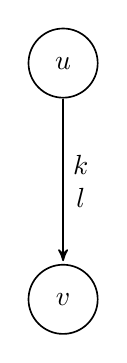
\begin{tikzpicture}[->,>=stealth',shorten >=1pt,auto,node distance=3cm,
                    semithick]
  \tikzstyle{every state}=[fill=white,text=black]

  \node[state] (1) {$u$};
  \node[state] (2) [below of=1] {$v$};

  \path 	(1) 	edge node[align=center] {$k$\\$l$} (2);
\end{tikzpicture}
\captionof{subfigure}{Case where both $u_e$ and $l_e$ are finite constants.}
\label{fig:case1}
\end{minipage}%
\quad
\begin{minipage}{.22\textwidth}
\centering
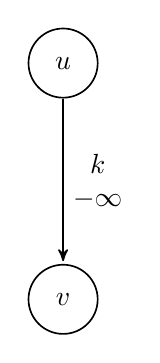
\begin{tikzpicture}[->,>=stealth',shorten >=1pt,auto,node distance=3cm,
                    semithick]
  \tikzstyle{every state}=[fill=white,text=black]

  \node[state] (1) {$u$};
  \node[state] (2) [below of=1] {$v$};

  \path 	(1) 	edge node[align=center] {$k$\\$-\infty$} (2);
\end{tikzpicture}
\captionof{subfigure}{Case where both $u_e$ are a finite constant and $l_e$ is
  negative infinite.}
\label{fig:case2}
\end{minipage}%
\quad
\begin{minipage}{.22\textwidth}
\centering
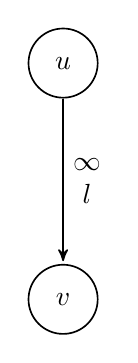
\begin{tikzpicture}[->,>=stealth',shorten >=1pt,auto,node distance=3cm,
                    semithick]
  \tikzstyle{every state}=[fill=white,text=black]

  \node[state] (1) {$u$};
  \node[state] (2) [below of=1] {$v$};

  \path 	(1) 	edge node[align=center] {$\infty$\\$l$} (2);
\end{tikzpicture}
\captionof{subfigure}{Case where $u_e$ is infinite and $l_e$ is a constant.}
\label{fig:case3}
\end{minipage}%
\quad
\begin{minipage}{.22\textwidth}
\centering
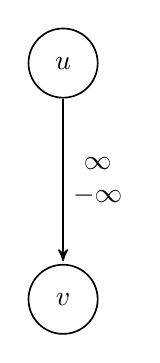
\begin{tikzpicture}[->,>=stealth',shorten >=1pt,auto,node distance=3cm,
                    semithick]
  \tikzstyle{every state}=[fill=white,text=black]

  \node[state] (1) {$u$};
  \node[state] (2) [below of=1] {$v$};

  \path 	(1) 	edge node[align=center] {$\infty$\\$-\infty$} (2);
\end{tikzpicture}
\captionof{subfigure}{Case where $u_e$ are infinite and $l_e$ is negative
  infinite.}
\label{fig:case4}
\end{minipage}%


\caption{The different cases for vertices and edges.}
\label{fig:cases}
\end{figure}

\subsection{Exercise 3.1}
The only case we need to handle here is case 4, as seen in Figure
\ref{fig:case4}.  If we have a graph $G=(V,E)$ where $V=\{u,v\}$ and
$E=\{(u,v)\}$, with $l_{(u,v)} = -\infty$ and $u_{(u,v)}=\infty$ we can view the
negative $l$ capacity as an edges ability to carry flow in the reverse
direction. But inserting an anti-parallel edge $(v,u)$ with $u_{(v,u)} =
\infty$, this will make the $l$ value for both edges equal to 0. Figure
\ref{fig:3_1_ex1} shows the example graph before and after this operation.

\begin{figure}[H]
\centering
\begin{minipage}{.25\textwidth}
\centering
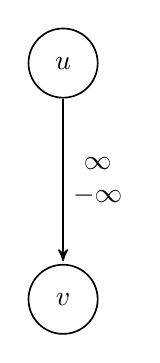
\begin{tikzpicture}[->,>=stealth',shorten >=1pt,auto,node distance=3cm,
                    semithick]
  \tikzstyle{every state}=[fill=white,text=black]

  \node[state] (1) {$u$};
  \node[state] (2) [below of=1] {$v$};

  \path 	(1) 	edge node[align=center] {$\infty$\\$-\infty$} (2);
\end{tikzpicture}
\captionof{subfigure}{The initial graph $G$ with two vertices and on edge.}
\label{fig:3_1_ex1a}
\end{minipage}%
$\Longrightarrow$
\begin{minipage}{.25\textwidth}
\centering
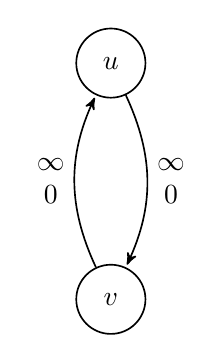
\begin{tikzpicture}[->,>=stealth',shorten >=1pt,auto,node distance=3cm,
                    semithick]
  \tikzstyle{every state}=[fill=white,text=black]


  \node[state] (1) {$u$};
  \node[state] (2) [below of=1] {$v$};

  \path 	(1) 	edge[bend left=25] node[align=center] {$\infty$\\$0$} (2)
		(2)	edge[bend left=25] node[align=center] {$\infty$\\$0$} (1);
\end{tikzpicture}
\captionof{subfigure}{The resulting graph $G$ with 2 vertices and 2 edges.}
\label{fig:3_1_ex1b}
\end{minipage}

\caption{The result of the first part of the operation.}
\label{fig:3_1_ex1}
\end{figure}

Since we cannot have anti-parallel edges we will insert an extra vertex and
connect one of the edges to this vertex and add a new edge. The new vertex $w$
shall have a demand $b = 0$ so as to not consume or produce any additional
flow. The edge $(v,u)$ shall be changed to $(v,w)$ and a new edge with $(w,u)$
shall be introduced with the same capacities but with cost $c(w,u) = 0$. Figure
\ref{fig:3_1_ex2} Illustrates this example.

\begin{figure}[H]
\centering
\begin{minipage}{.25\textwidth}
\centering
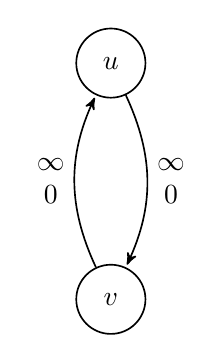
\begin{tikzpicture}[->,>=stealth',shorten >=1pt,auto,node distance=3cm,
                    semithick]
  \tikzstyle{every state}=[fill=white,text=black]


  \node[state] (1) {$u$};
  \node[state] (2) [below of=1] {$v$};

  \path 	(1) 	edge[bend left=25] node[align=center] {$\infty$\\$0$} (2)
		(2)	edge[bend left=25] node[align=center] {$\infty$\\$0$} (1);
\end{tikzpicture}
\captionof{subfigure}{The graph $G$ after the first operation.}
\label{fig:3_1_ex2a}
\end{minipage}%
$\Longrightarrow$
\begin{minipage}{.25\textwidth}
\centering
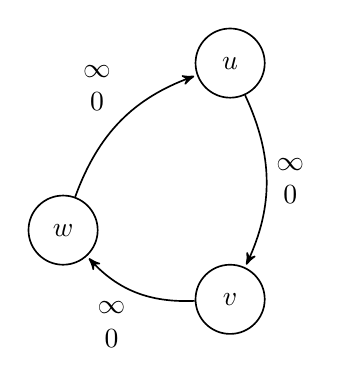
\begin{tikzpicture}[->,>=stealth',shorten >=1pt,auto,node distance=3cm,
                    semithick]
  \tikzstyle{every state}=[fill=white,text=black]


  \node[state] (1) {$u$};
  \node[state] (2) [below of=1] {$v$};
  \node[state] (3) [below left of=1] {$w$};

  \path 	(1) 	edge[bend left=25] node[align=center] {$\infty$\\$0$} (2)
		(2)	edge[bend left=25] node[align=center] {$\infty$\\$0$} (3)
                (3)     edge[bend left=25] node[align=center] {$\infty$\\$0$} (1);
\end{tikzpicture}
\captionof{subfigure}{The final graph $G$ at the end of the procedure.}
\label{fig:3_1_ex2b}
\end{minipage}

\caption{The result of the entire operation.}
\label{fig:3_1_ex2}
\end{figure}

\subsection{Exercise 3.2}

For this part we need only consider case 2 as seen in Figure \ref{fig:case2}
since we have already solved this for case 4 in the previous question.  This
problem is solvable using the exact same method as above, only the $u_e$ values
are different. The reduction can be seen in Figure \ref{fig:3_2_ex1}

\begin{figure}[H]
\centering
\begin{minipage}{.25\textwidth}
\centering
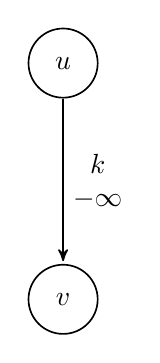
\begin{tikzpicture}[->,>=stealth',shorten >=1pt,auto,node distance=3cm,
                    semithick]
  \tikzstyle{every state}=[fill=white,text=black]

  \node[state] (1) {$u$};
  \node[state] (2) [below of=1] {$v$};

  \path 	(1) 	edge node[align=center] {$k$\\$-\infty$} (2);
\end{tikzpicture}
\captionof{subfigure}{The graph $G$ in the beginning.}
\label{fig:3_2_ex1a}
\end{minipage}%
$\Longrightarrow$
\begin{minipage}{.25\textwidth}
\centering
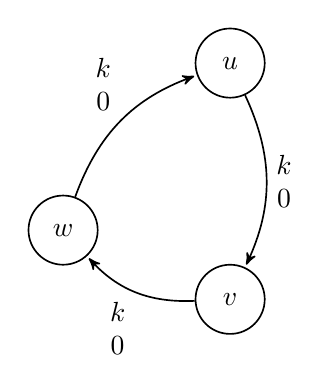
\begin{tikzpicture}[->,>=stealth',shorten >=1pt,auto,node distance=3cm,
                    semithick]
  \tikzstyle{every state}=[fill=white,text=black]


  \node[state] (1) {$u$};
  \node[state] (2) [below of=1] {$v$};
  \node[state] (3) [below left of=1] {$w$};

  \path 	(1) 	edge[bend left=25] node[align=center] {$k$\\$0$} (2)
		(2)	edge[bend left=25] node[align=center] {$k$\\$0$} (3)
                (3)     edge[bend left=25] node[align=center] {$k$\\$0$} (1);
\end{tikzpicture}
\captionof{subfigure}{The final graph $G$ at the end of the procedure.}
\label{fig:3_2_ex1b}
\end{minipage}

\caption{The result of the entire operation.}
\label{fig:3_2_ex1}
\end{figure}

\subsection{Exercise 3.3}

In the two previous questions we did this for case 2 and 4 (Figure
\ref{fig:case2} and \ref{fig:case4}). We will now pay attention to case 1 and 3
(Figure \ref{fig:case1} and \ref{fig:case3}.) It is worth noticing that with
these two casses there is no requirement that the finite constant $l$ be
negative, it might also be positive.

\subsection{Exercise 3.4}
\subsection{Exercise 3.5 (Optional)}


\newpage
\appendix
% Bibliography
\bibliographystyle{plain}
\bibliography{bib}

\end{document}
